\documentclass[journal]{IEEEtran}
\renewcommand{\IEEEkeywordsname}{Keywords}

\usepackage[italian]{babel}
\usepackage[utf8]{inputenc}
\usepackage[T1]{fontenc}

\setlength{\marginparwidth}{2cm}
\usepackage[italian, textsize=small, textwidth=2cm]{todonotes}

\usepackage{hyperref}
\usepackage{url}
\usepackage{tikz}
\usetikzlibrary{shapes.geometric, arrows}
\usepackage[dvipsnames]{xcolor}
\usepackage{listings}
\renewcommand{\lstlistingname}{Codice}

\usepackage{amsmath}
\newcommand{\bigo}[1]{\ensuremath{O\left({#1}\right)}}
\usepackage{booktabs}
\usepackage{mathtools}
\DeclarePairedDelimiter\bra{\langle}{\rvert}
\DeclarePairedDelimiter\ket{\lvert}{\rangle}
\DeclarePairedDelimiterX\braket[2]{\langle}{\rangle}{#1\,\delimsize\vert\,\mathopen{}#2}
\usepackage{amsmath, amssymb}

\usepackage{listings,newtxtt,xcolor}
% Define custom colors
\definecolor{keywordcolor}{rgb}{0.1, 0.1, 0.75}  % Blue for keywords
\definecolor{stringcolor}{rgb}{0.1, 0.5, 0.1}    % Green for strings
\definecolor{commentcolor}{rgb}{0.5, 0.5, 0.5}   % Gray for comments
\definecolor{bgcolor}{rgb}{0.95, 0.95, 0.95}     % Light gray background

% Configure lstset for Python
\lstset{
    language=Python,                    % Set the language to Python
    backgroundcolor=\color{bgcolor},   % Background color for code
    basicstyle=\ttfamily\footnotesize, 
	keywordstyle=\color{keywordcolor}\bfseries, % Keywords in bold blue
    stringstyle=\color{stringcolor},   % Strings in green
    commentstyle=\color{commentcolor}\itshape, % Comments in italic gray
    identifierstyle=,                  % Default identifier style
    showstringspaces=false,            % Don't show spaces in strings
    numbers=left,                      % Line numbers on the left
    numberstyle=\tiny\color{commentcolor}, % Line number style
    numbersep=5pt, % Spaziatura dei numeri di riga
    %  frame=single, % Cornice intorno al blocco di codice
    % framerule=0.1pt,
    linewidth=0.98\columnwidth,
    stepnumber=1,                      % Line numbers increment by 1
    tabsize=4,                         % Tab size
    breaklines=true,                   % Automatically break long lines
    breakatwhitespace=true,            % Break lines only at whitespace
    frame=none,                      % Draw a box around the code
    captionpos=b,                      % Caption position: b for bottom
    escapeinside={(*@}{@*)},           % Escape to LaTeX between (*@ and @*)
}

\usepackage{graphicx}
\graphicspath{{sections/images/}}

\begin{document}

\title{Quantum Hadamard Edge Detection}

\author{\IEEEauthorblockN{Manuel Di Agostino}
\IEEEauthorblockA{\textit{Università degli studi di Parma} \\
Parma, Italia\\
manuel.diagostino@studenti.unipr.it}\\

\IEEEauthorblockN{Leonardo Ongari}
\IEEEauthorblockA{\textit{Università degli studi di Parma} \\
Cremona, Italia \\
leonardo.ongari@studenti.unipr.it}
}

\maketitle

\begin{abstract}
	Il rilevamento dei bordi è un processo fondamentale nell'estrazione delle 
	caratteristiche di un'immagine ed è ampiamente utilizzato per analizzare 
	la struttura degli oggetti rappresentati. Tuttavia, con l'aumento della 
	risoluzione delle immagini, i metodi classici affrontano significative 
	sfide computazionali a causa delle operazioni pixel-per-pixel necessarie. 
	Il \emph{Quantum Image Processing}, offre il potenziale per accelerazioni 
	esponenziali in determinati scenari, sfruttando algoritmi e rappresentazioni 
	in forma quantistica. Questo articolo esplora l'applicazione dell'algoritmo 
	\emph{Quantum Hadamard Edge Detection}, implementato utilizzando la 
	rappresentazione \emph{Quantum Probability Image Encoding}. 
	Utilizzando i principi quantistici e il framework Qiskit, si analizzano 
	i vantaggi e le prospettive di questo nuovo approccio per il rilevamento dei bordi.
\end{abstract}

\begin{IEEEkeywords}
Rilevamento dei bordi, Quantum computing, Sobel.
\end{IEEEkeywords}

\section{Introduzione}

L'identificazione dei bordi è una tecnica fondamentale nell'elaborazione delle
immagini, utilizzata per individuare i contorni degli oggetti e le variazioni di
intensità in una scena. Questa metodologia rappresenta una componente cruciale
in numerosi ambiti, dalla computer vision alla robotica, fino all'analisi medica
delle immagini. Nonostante i progressi significativi nell'elaborazione classica
delle immagini, l'aumento della risoluzione e della complessità dei dati visivi
ha portato a sfide computazionali sempre maggiori, rendendo spesso i metodi
tradizionali onerosi in termini di tempo e risorse.

Nei primi anni '60, i filtri di Sobel \cite{SobelFeldman1968IsotropicGradient} e Prewitt furono introdotti come i primi metodi strutturati per il rilevamento dei bordi. Entrambi basati su operatori convolutivi, questi algoritmi utilizzano maschere discrete per approssimare il gradiente di intensità in un'immagine, rilevando così variazioni significative nei livelli di grigio. Sebbene semplici ed efficienti, essi risultano sensibili al rumore e con conseguente difficoltà nel gestire bordi sfumati. Negli anni '80, l'algoritmo di Canny~\cite{CannyPaper} rappresentò una svolta significativa grazie all'introduzione di un approccio più sofisticato al rilevamento dei bordi; ancora oggi, rimane uno tra i metodi più utilizzati. Con l'avanzare della tecnologia e l'aumento della potenza computazionale, il rilevamento dei bordi ha beneficiato dell'utilizzo di tecniche basate sull'intelligenza artificiale, come le \emph{reti neurali convoluzionali} (CNN).

\section{Background}\label{sec:background}

\subsection{Soluzioni classiche}
Le tecniche classiche per la rilevazione dei contorni prevedono l'utilizzo di 
kernel specifici, che permettono di calcolare nuovi valori di intensità per i pixel 
dell'immagine. Tra i metodi più famosi vi è sicuramente l'operatore di Sobel, 
che si può descrivere tramite l'applicazione di 2 kernel all'immagine originale:
\[
\mathbf{G_x} =
\begin{bmatrix}
+1 & 0 & -1 \\
+2 & 0 & -2 \\
+1 & 0 & -1
\end{bmatrix}
, \, 
\mathbf{G_y} =
\begin{bmatrix}
+1 & +2 & +1 \\
0 & 0 & 0 \\
-1 & -2 & -1
\end{bmatrix}
\]

Un'altra opzione, forse tra le più utilizzate al giorno d'oggi, è l'operatore di
Canny. Questo metodo ha un funzionamento del tutto analogo al precedente, ma
aggiunge meccanismi per la riduzione del rumore nell'immagine
\cite{digital_image_processing}. La complessità di queste tecniche è lineare
rispetto al numero di pixel totali dell'immagine, dato che è necessaria una
visita completa. In questo progetto verrà mostrato come, dopo una prima fase di
preparazione, è possibile risolvere il problema in tempo costante $\bigo{1}$.

\subsection{Sistemi quantistici}

Analogamente a quanto accade nei computer classici, i computer quantistici utilizzano i \textbf{quantum bit}, chiamati \emph{qubit}. I qubit rappresentano la più piccola unità di informazione e sono implementati attraverso sistemi quantistici bidimensionali. Le quantità fisiche comunemente usate per questo scopo includono lo spin di una particella o gli stati eccitati degli atomi.

Assemblando più qubit, è possibile costruire sistemi quantistici la cui dinamica è descritta da spazi vettoriali complessi. Un sistema composto da un singolo qubit è completamente descritto da
\begin{equation}
	\ket{\psi} = \begin{bmatrix}
		\alpha\\ \beta
	\end{bmatrix} = \alpha \ket{0} + \beta \ket{1},\quad \alpha,\beta \in
	\mathbb{C}
	\label{eq:1-qubit-state}
\end{equation}

Mentre un bit classico può assumere soltanto uno tra due possibili valori
(generalmente 0 e 1), un bit quantistico è denotato da una combinazione lineare
dei suoi stati base, pesata dai coefficienti complessi $\alpha$ e $\beta$. Tali
coefficienti sono detti \emph{ampiezze di probabilità} e rispettano la seguente:
\begin{equation}
	|\alpha|^2 + |\beta|^2 = 1
	\label{eq:qubit-prob}
\end{equation}

Per descrivere lo stato di un sistema quantistico composto da più qubit, è
necessario effettuare un'operazione chiamata \emph{prodotto tensoriale} tra i
singoli stati coinvolti. Ad esempio, considerati i vettori di stati
\[
\ket{\psi_1} = \begin{bmatrix} a_1 \\ a_2 \end{bmatrix}, \quad \ket{\psi_2} = \begin{bmatrix} b_1 \\ b_2 \end{bmatrix},
\]
il loro prodotto tensore è definito come:
\begin{equation}
\ket{\psi_1} \otimes \ket{\psi_2}
= \begin{bmatrix}
a_1 \begin{bmatrix} b_1 \\ b_2 \end{bmatrix} \\
a_2 \begin{bmatrix} b_1 \\ b_2 \end{bmatrix}
\end{bmatrix} =
\begin{bmatrix}
a_1 b_1 \\ a_1 b_2 \\ a_2 b_1 \\ a_2 b_2
\end{bmatrix}.
\label{eq:tensor-prod}
\end{equation}
Equivalentemente, può essere scritto come $\ket{\psi_1}\ket{\psi_2} \text{ o } \ket{\psi_1
\psi_2}$.

\todo{Se serve, parlare dell'entanglement}

\subsection{Circuiti quantistici}

Analogamente a quanto accade nei circuiti digitali classici, i circuiti
quantistici eseguono calcoli manipolando le informazioni immagazzinate nei
qubit. Questo viene realizzato attraverso dispositivi chiamati \textbf{quantum
gate} (\emph{porte quantistiche}), che sono l'equivalente quantistico delle porte logiche classiche
ma operano secondo i principi della meccanica quantistica. L'applicazione di una
matrice \emph{complessa unitaria} ad uno stato quantistico modella matematicamente l'azione di un
gate su di esso. Formalmente, data $U \in \mathcal{M}_{n \times n}(\mathbb{C})$
l'unitaria associata ad una porta logica e dato lo stato $\ket{\psi} \in
\mathbb{C}^n$, lo stato risultante dall'applicazione è definito come:
\begin{equation}
	\ket{\psi'} = U\ket{\psi}
	\label{eq:gate-res-state}
\end{equation}

\subsubsection*{Gate rilevanti}

Di seguito sono descritti alcuni gate quantistici di rilevante importanza. Tra
questi, figurano i \emph{gate di Pauli}.
\begin{itemize}
	\item \textbf{X} (NOT quantistico): trasforma lo stato $\ket{0}$ in $\ket{1}$
	e viceversa;
	\[
		X =\begin{bmatrix}
			0 & 1\\
			1 & 0
		\end{bmatrix}
	\]
	\item \textbf{Y}: combina una rotazione coniugata complessa con un'inversione, utile per applicazioni che coinvolgono trasformazioni nel piano complesso;
	\[
		Y =\begin{bmatrix}
			0 & -i\\
			i & 0
		\end{bmatrix}
	\]
	\item \textbf{Z}: applica una fase negativa allo stato $\ket{1}$ senza influenzare $\ket{0}$.
	\[
		Z =\begin{bmatrix}
			1 & 0\\
			0 & -1
		\end{bmatrix}
	\]
\end{itemize}

Altro gate fondamentale è quello di \emph{Hadamard}\label{txt:hadamard}, essenziale per creare stati
di sovrapposizione. L'unitaria che lo rappresenta è:
\[
	H = \frac{1}{\sqrt 2}\begin{bmatrix}
			1 & 1\\
			1 & -1
		\end{bmatrix}
\]
In particolare, si noti che:
\begin{align}
	H\ket{0} &= \frac{\ket{0} + \ket{1}}{\sqrt 2} =: \ket{+} \\
	H\ket{1} &= \frac{\ket{0} - \ket{1}}{\sqrt 2} =: \ket{-}
\end{align}

Il \emph{Controlled-NOT} (CNOT) è un'operazione che coinvolge due qubit, dove
uno funge da controllo sull'altro. Il gate inverte lo stato del qubit target se il qubit di controllo è $\ket{1}$. La sua matrice è:
\[
	\text{CNOT} = \begin{bmatrix}
		1 & 0 & 0 & 0\\
		0 & 1 & 0 & 0\\
		0 & 0 & 0 & 1\\
		0 & 0 & 1 & 0
	\end{bmatrix}
\]
\subsection{Quantum Image Processing}

La \textbf{Quantum Image Processing} (\emph{processamento quantistico
dell'immagine}) si concentra sullo sviluppo di algoritmi in grado di codificare immagini all’interno di circuiti quantistici e di processarle utilizzando operazioni quantistiche. 

\subsubsection*{Rappresentazione delle immagini}\label{sec:img-rappr} Tra le varie tecniche proposte negli
ultimi anni, la \textbf{Quantum Probability Image Encoding (QPIE)} \cite{qpie} utilizza le ampiezze di probabilità di uno stato quantistico per memorizzare i valori dei pixel di un'immagine classica. Dati $n$ qubit, essa consente di rappresentare un'immagine in toni di grigio di $2^n$ pixel tramite una superposizione di stati. In generale, il numero di qubit necessari è calcolato tramite:
\begin{equation}
	n = \lceil{\log_2{N}}\rceil
	\label{eq:qpie-n-qubit}
\end{equation}

Come mostrato in Fig.
\ref{fig:bw-4x4-img},
ogni pixel può essere numerato utilizzando stringhe binarie ($00,01,10,11$);
l'intera immagine è quindi
rappresentabile come una matrice $2\times2$ delle intensità di colore. In questa
notazione, il singolo termine $I_{i}$ corrisponde all'intensità del pixel in posizione
$(x,y)$ (rispetto all'angolo in alto a sinistra), tale per cui $i = {xy}_{10}$.
\begin{figure}[ht!]
    \centering
    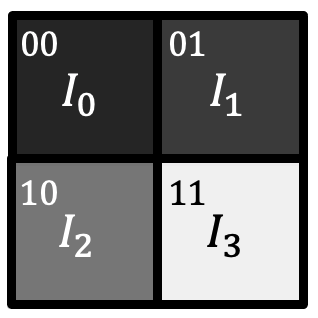
\includegraphics[width=0.5\columnwidth]{classical_repr.png}
		\caption{Rappresentazione di un'immagine B\&W 2x2 pixel.}
    \label{fig:bw-4x4-img}
\end{figure}

Per rappresentare l'immagine come una superposizione di stati base, è necessario
che venga rispettata l'Eq. \ref{eq:qubit-prob}; bisogna infatti normalizzare le singole intensità come segue:
\begin{equation}
	c_i = \frac{I_i}{\sqrt{\sum_{k}^{}{I_{k}^2}}}
	\label{eq:intensities-norm}
\end{equation}
In Fig. \ref{fig:bw-4x4-img-qpie}
viene mostrato il risultato della normalizzazione.
\begin{figure}[ht!]
    \centering
    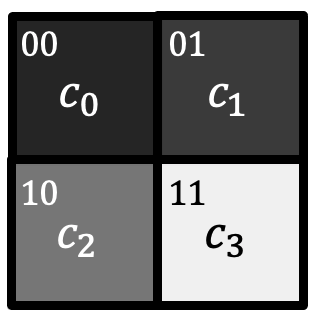
\includegraphics[width=0.5\columnwidth]{QPIE_repr.png}
		\caption{Rappresentazione della Fig. \ref{fig:bw-4x4-img} tramite QPIE.}
    \label{fig:bw-4x4-img-qpie}
\end{figure}

L'immagine può quindi essere scritta come:
\begin{equation*}
	\ket{\text{Img}}
		= c_0 \ket{00} + c_1 \ket{01} + c_2 \ket{10} + c_3 \ket{11}
	\label{eq:qpie-img-2qubit}
\end{equation*}
che generalizzata a $n$ qubit diventa:
\begin{equation}
	\ket{\text{Img}}
		= \sum_{i=1}^{2^n} c_i \ket{i}
	\label{eq:qpie-img}
\end{equation}


\subsection{Quantum Hadamard Edge Detection}

L'algoritmo di \textbf{Quantum Hadamard Edge Detection (QHED)} \cite{qpie} rappresenta il
fulcro di questo progetto. L'idea alla base è quella di utilizzare il gate di
Hadamard. Come mostrato nella Sottosez.
\ref{sec:img-rappr}, esso trasforma
$\ket{0}$ in $\ket{+}$ e, in particolare, $\ket{1}$ in $\ket{-}$. Inoltre, in
base alla Eq. \ref{eq:qpie-img}, ogni pixel può essere identificato
da una stringa binaria del tipo 
\[
	\ket{b_{n-1}b_{n-2}\ldots b_1b_0},\quad b_i \in {0,1}
\]
Per pixel orizzontalmente adiacenti presi a due a due, le stringhe sono:
\[
	\ket{b_{n-1}b_{n-2}\ldots b_10}, \ket{b_{n-1}b_{n-2}\ldots b_11}
\]
ossia si differenziano soltanto per l'ultimo qubit più a destra, denotato con $q_0$.

Applicando il gate $H$ a $q_0$, si ottiene una trasformazione la cui unitaria è
rappresentata da:
\begin{equation*}
	I_{2^{n-1}} \otimes H_0 = \frac{1}{\sqrt 2}\begin{bmatrix}
		1 & 1 & 0 & 0 & \ldots & 0 & 0\\
		1 & -1 & 0 & 0 & \ldots & 0 & 0\\
		0 & 0 & 1 & 1 & \ldots & 0 & 0\\
		0 & 0 & 1 & -1 & \ldots & 0 & 0\\
		\vdots & \vdots & \vdots & \vdots & \ddots & \vdots & \vdots\\
		0 & 0 & 0 & 0 & \ldots & 1 & 1\\
		0 & 0 & 0 & 0 & \ldots & 1 & -1\\
	\end{bmatrix}
\end{equation*}
Se a questo punto tale trasformazione è applicata allo stato che codifica
l'immagine nella notazione QPIE (Eq. \ref{eq:qpie-img}), si
ottiene:
\begin{equation}\label{eq:had-applied-simple}
	(I_{2^{n-1}} \otimes H_0) \cdot \begin{bmatrix}
		c_0\\ c_1\\ c_2\\ c_3\\ \vdots\\ c_{N-2}\\ c_{N-1}
	\end{bmatrix} = \frac{1}{\sqrt 2} \begin{bmatrix}
		c_0+c_1\\ c_0-c_1\\ c_2+c_3\\ c_2-c_3\\ \vdots\\ c_{N-2}+c_{N-1}\\ c_{N-2}-c_{N-1}
	\end{bmatrix}
\end{equation}
Si noti che ciò permette di esplicitare il gradiente di coppie di pixel adiacenti, in corrispondenza dei coefficienti in posizione \emph{pari} nel vettore di stato risultante ($(0,1), (2,3), \ldots$). Lo stato dell'Eq. \ref{eq:had-applied-simple} può essere riscritto come:
\begin{align*}
	&\frac{1}{\sqrt 2} \begin{bmatrix}
	c_0+c_1\\ c_0-c_1\\ c_2+c_3\\ c_2-c_3\\ \vdots\\ c_{N-2}+c_{N-1}\\ c_{N-2}-c_{N-1}
\end{bmatrix}\\
	&=\frac{1}{\sqrt 2} 
\left(
\begin{bmatrix}
c_0+c_1\\ 0\\ c_2+c_3\\ 0\\ \vdots\\ c_{N-2}+c_{N-1}\\ 0
\end{bmatrix} + \begin{bmatrix}
0\\ c_0-c_1\\ 0\\ c_2-c_3\\ \vdots\\ 0\\ c_{N-2}-c_{N-1}
\end{bmatrix}
\right)\\
	&=\frac{1}{\sqrt 2} (\ket{\text{sum}} \otimes \ket{0}
		+ \ket{\text{dif}} \otimes \ket{1})
\end{align*}
da cui si evince che, misurando il circuito condizionato sul fatto che $q_0$ sia nello stato $\ket{1}$, è possibile ottenere i gradienti attraverso un'analisi statistica. Per ottenere i gradienti orizzontali tra coppie di pixel \emph{dispari} ($(1,2), (3,4), \ldots$), è possibile effettuare una permutazione preliminare del vettore dei qubit:
\begin{equation}\label{eq:perm}
	(c_0, c_1, \ldots, c_{N-1})^T \mapsto (c_1, c_2, \ldots, c_{N-1}, c_0)^T
\end{equation}
e procedere poi con l'applicazione del circuito.

\subsubsection*{Variazione del QHED}

Per evitare la permutazione (\ref{eq:perm}), in questo progetto
è impiegata una
versione estesa del QHED. Essa prevede l'utilizzo di un qubit aggiuntivo $q_a$,
utilizzato per creare ridondanza di informazione. Inizialmente, il qubit
aggiuntivo è inizializzato in $\ket{0}$; segue un'applicazione del gate $H$,
permettendo di ottenere lo stato:
\begin{equation*}
	\ket{\text{Img}} \otimes 
		\frac{(\ket{0} + \ket{1})}{\sqrt 2} =
		\frac{1}{\sqrt 2} \begin{bmatrix}
			c_0\\c_0\\c_1\\c_1\\c_2\\c_2\\\vdots\\c_{N-1}\\c_{N-1}
		\end{bmatrix}
\end{equation*}
Successivamente, si applica la matrice di shift:
\begin{equation*}
	D_{2^{n+1}} = \begin{bmatrix}
		0 & 1 & 0 &\ldots& 0 \\
		0 & 0 & 1 &\ldots& 0 \\
		\vdots & \vdots & \vdots & \ddots & \vdots \\
		0 & 0 &\ldots & 0 & 1\\
		1 & 0 &\ldots & 0 & 0\\
	\end{bmatrix}
	\label{eq:eq-perm-matrix}
\end{equation*}
per ottenere il nuovo stato:
\begin{equation*}
	D_{2^{n+1}} \cdot \begin{bmatrix}
		c_0\\c_0\\c_1\\c_1\\c_2\\c_2\\\vdots\\c_{N-1}\\c_{N-1}
	\end{bmatrix} = \begin{bmatrix}
		c_0\\c_1\\c_1\\c_2\\c_2\\\vdots\\c_{N-1}\\c_{N-1}\\c_0
	\end{bmatrix}
	\label{eq:perm-state}
\end{equation*}
A questo punto, viene applicato il gate $H$ a $q_a$; questo permette
di ottenere, in un'unico passo, sia i gradienti relativi alle coppie \emph{pari} sia quelli relativi alle coppie \emph{dispari}:
\begin{equation*}
	(I_{2^n} \otimes H_a) \cdot \begin{bmatrix}
		c_0\\c_1\\c_1\\c_2\\c_2\\\vdots\\c_{N-1}\\c_{N-1}\\c_0
	\end{bmatrix} = \begin{bmatrix}
		c_0+c_1\\c_0-c_1\\c_1+c_2\\c_1-c_2\\c_2+c_3\\c_2-c_3\\\vdots\\c_{N-1}+c_0\\c_{N-1}-c_0
	\end{bmatrix}
	\label{eq:h-to-adj-qubit}
\end{equation*}
In ultimo è possibile ottenere, tramite analisi statistica, il valore di tutti i
gradienti orizzontali per le misurazioni in cui $q_a$ è nello stato $\ket{1}$.

% \subsection{Modellazione del rumore}

\section{Implementazione}\label{sec:implementazione}

\subsection{Modellazione circuito}
Come accennato nella Sez. \ref{sec:background}, la rappresentazione 
delle immagini viene implementata attraverso la tecnica QPIE. 
Per farlo, si utilizza una matrice associata all'immagine di partenza
i cui elementi corrispondono ai valori d'intensità dei pixel.
Su questa matrice viene effettuato un processo di normalizzazione.
Il risultato è un vettore di stato, composto da ampiezze di
probabilità relative allo stato quantistico del sistema. In Fig.~\ref{fig:16x16intensity_img} 
è mostrata un'immagine di 
dimensione $16 \times 16$ dopo la normalizzazione. Ogni pixel 
con valore ``alto'' rappresenta un possibile risultato della misurazione sul 
circuito associato. Il colore indica l'ampiezza di probabilità relativa alla 
misurazione del pixel, che a sua volta rappresenta una possibile configurazione 
del circuito.

Dato un vettore di stato composto da $2^n$ elementi, 
il passo successivo consiste nella creazione di un circuito a $n+1$ qubit, 
compreso quello ausiliario o \textit{ancilla qubit}.
La costruzione avviene tramite applicazione di procedure Qiskit \textit{built-in} 
all'oggetto che rappresenta il circuito.
Nel Cod. \ref{cod:circuit} vengono mostrate le operazioni svolte durante
questa fase, oltre all'applicazione dei gate Hadamard e della matrice 
di shift $D_{2^{n+1}}$.

\begin{figure}
    \centering
    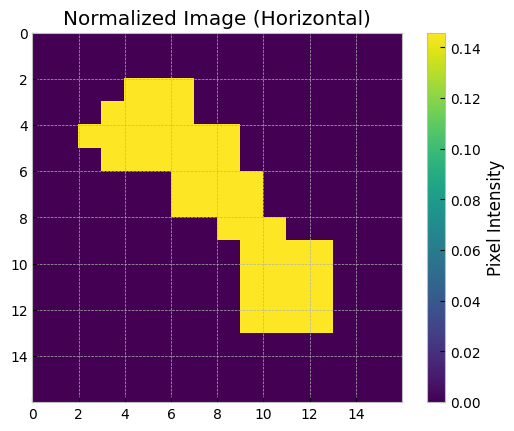
\includegraphics[width=0.4\textwidth]{16x16.png}
    \caption{Immagine normalizzata (ampiezze di probabilità).}
    \label{fig:16x16intensity_img}
\end{figure}

\begin{lstlisting}[language=Python, 
    caption={Creazione dei circuiti per lo scan orizzontale e verticale.}, label=cod:circuit]
# Convert the raw pixel values to probability amplitudes
def amplitude_encode(img_data):
    
    # Calculate the RMS value
    rms = np.sqrt(np.sum(np.sum(img_data**2, axis=1)))
    
    # Create normalized image
    image_norm = []
    for arr in img_data:
        for ele in arr:
            image_norm.append(ele / rms)
        
    # Return the normalized image as a numpy array
    return np.array(image_norm)
# Initialize some global variable for number of qubits
data_qb = math.floor(math.log2(height * width))
anc_qb = 1
total_qb = data_qb + anc_qb

# Initialize the amplitude permutation unitary
D2n_1 = np.roll(np.identity(2**total_qb), 1, axis=1)

# Create the circuit for horizontal scan
qc_h = QuantumCircuit(total_qb)
qc_h.initialize(image_norm_h, range(1, total_qb))
qc_h.h(0)
qc_h.unitary(D2n_1, range(total_qb))
qc_h.h(0)
display(qc_h.draw('mpl', fold=-1))

# Create the circuit for vertical scan
qc_v = QuantumCircuit(total_qb)
qc_v.initialize(image_norm_v, range(1, total_qb))
qc_v.h(0)
qc_v.unitary(D2n_1, range(total_qb))
qc_v.h(0)
display(qc_v.draw('mpl', fold=-1))

# Combine both circuits into a single list
circ_list = [qc_h, qc_v]
\end{lstlisting} 

\begin{figure}[ht]
    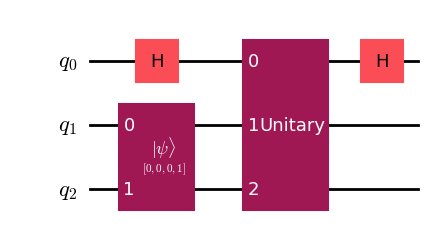
\includegraphics[width=0.4\textwidth]{circuit.png}
    \caption{Circuito per scan orizzontale su immagine $2 \times 2$.}
    \label{fig:circuit}
\end{figure}

Il circuito ottenuto per un'immagine $2 \times 2$ è mostrato in Fig.~\ref{fig:circuit}.
Come si può notare, l'operazione relativa alla matrice di shift (chiamata anche
\emph{decrement gate}) è 
rappresentata come una black-box di cui non si conoscono i dettagli.
È possibile, tuttavia, utilizzare una rappresentazione più a basso livello 
composta solo da porte logiche $H$, $X$, $CX$ e $CCX$ (Toffoli gate).
Questa casistica è presentata solo per immagini di piccole dimensioni: altre versioni
introdurrebbero troppo rumore e i risultati realistici non sarebbero quindi 
interessanti. La parte di circuito a sinistra della barriera
corrisponde alla preparazione dello stato $\ket{\psi}$: in questo caso, si tratta 
di impostare a 1 il valore del qubit $q_1$.
In Fig. \ref{fig:2x2-original} e \ref{fig:circuito-2x2} viene mostrata l'immagine 
originale e la relativa implementazione a basso livello.

\begin{figure}[ht]
	\centering
	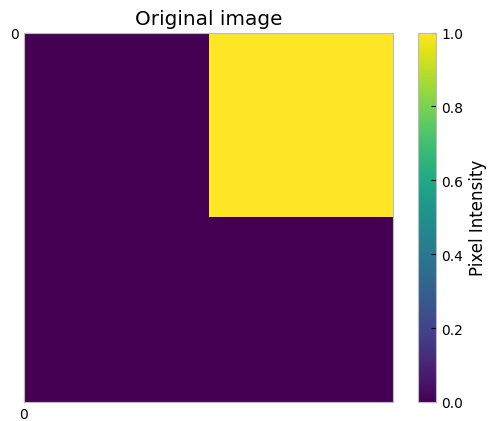
\includegraphics[width=0.6\columnwidth]{2x2-original.png}
	\caption{Esempio di immagine $2\times2$.}\label{fig:2x2-original}
\end{figure}

\begin{figure}[ht]
    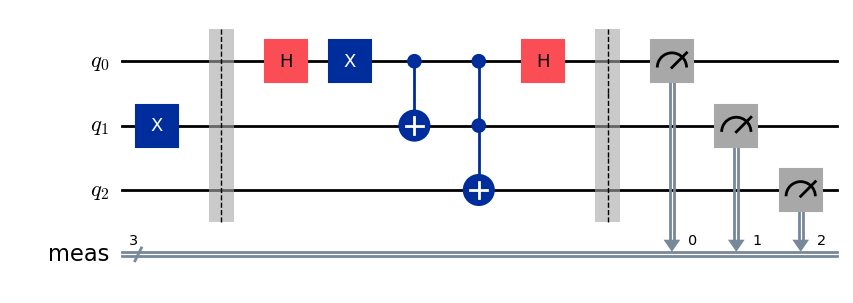
\includegraphics[width=0.4\textwidth]{low-level.png}
    \caption{Versione del circuito a basso livello.}
		\label{fig:circuito-2x2}
\end{figure}

\subsection{Simulazioni ideali}
Le misurazioni vengono svolte inizialmente tramite simulazione, utilizzando 
il framework \texttt{statevector\_simulator}. In questo meccanismo si lavora su 
una simulazione di un circuito quantistico ideale, ovvero senza effetti collaterali come
fluttuazioni termiche, imperfezioni delle porte quantistiche, interazione con l'ambiente 
o altre tipologie di \textit{rumore}.
In un'esecuzione realistica, tuttavia, occorre tenere in considerazione
tali problematiche che, molto spesso, complicano pesantemente
il circuito e richiedono tecniche non banali di \textit{mitigazione dell'errore}.

\subsection{Gestione degli errori}
Si possono eseguire delle misurazioni significative utilizzando modelli 
di rumore forniti dalla classe \texttt{NoiseModel} di Qiskit. 
Per farlo, ci si connette ad uno dei backend disponibili, per esempio 
\texttt{ibm\_kyiv} in questo caso. Da questo backend si estrapolano le 
informazioni necessarie all'esecuzione, ovvero:
\begin{itemize}
	\item \emph{noise model}: rappresenta il modello di rumore considerato;
    \item \emph{basis gates:} rappresentano le porte disponibili sull'hardware;
    \item \emph{coupling map:} rappresenta la disposizione fisica dei qubit sull'hardware.
\end{itemize}
Dopo aver definito queste proprietà, si prosegue con le misurazioni 
ripetute del circuito. Nel Cod. \ref{cod:noise} sono mostrati 
i comandi per estrarre le informazioni necessarie e per eseguire 
in maniera iterativa le misurazioni del circuito, salvando i risultati 
come statistiche da elaborare in una fase successiva.

\begin{lstlisting}[language=Python, 
caption={Estrapolazione del modello di rumore dal backend \texttt{ibm\_kyiv}.}, label=cod:noise]
service = QiskitRuntimeService(channel="ibm_quantum", token="<token>")
backend = service.backend("ibm_kyiv")
noise_model = NoiseModel.from_backend(backend)
coupling_map = backend.configuration().coupling_map
basis_gates = noise_model.basis_gates
# Unione dei circuiti in una lista unica
circ_list = [qc_h, qc_v]
# Array per memorizzare i risultati intermedi
results_list = []

# Iterazione per variare il numero di shots
for exponent in range(8, 20, 2):
    shots = 2 ** exponent
    print(f"Running simulation with {shots} shots...")
    
    # Simulazione
    result = backend.run(circ_list, shots=shots).result()
    
    # Estrazione conteggi
    counts_h = result.get_counts(qc_h)
    counts_v = result.get_counts(qc_v)
    
    # Salvataggio risultati 
    results_list.append({
        'shots': shots,
        'counts_h': counts_h,
        'counts_v': counts_v
    })
\end{lstlisting}

\section{Risultati}\label{sec:risultati}

\section{Implementazione}\label{sec:conclusione}


\bibliographystyle{IEEEtran}
\bibliography{main}

\end{document}
